\section{Algorithms}
%%%%%%%%%%%%%%%%%%%%%%%%%%%%%%%%%%%%%%%%%%%%%%%%%%%%%%%%%%%%%%%%%%%%%%%%%%%%%
\subsection{Hierarchical Optimistic Optimization Algorithm}
$\mathcal{X}$-armed stuff here.

%%%%%%%%%%%%%%%%%%%%%%%%%%%%%%%%%%%%%%%%%%%%%%%%%%%%%%%%%%%%%%%%%%%%%%%%%%%%%
\subsection{Zooming Algorithm}
When the number of arms is infinite, additional assumptions are needed
about the relationship between the arms. For instance, arms
that are \emph{close} should produce similar results. The Zooming
Algorithm is defined to work in any example where the arms form a
metric space. In each phase, certain arms are chosen to be
\emph{active}, and the algorithm chooses which arm to play from these
active arms.

The Zooming Algorithm is composed of multiple phases, each of which is
composed of $2^{i_{ph}}$ rounds, where $i_{ph}$ is the current phase
number. In a given round, you \emph{activate} an arm if that arm is
not covered by another arm. Each arm covers a radius defined by
$r_t(v):=\sqrt{8*i_{ph}/(2+n_t(v)))}$ where $v$ is the active arm, and
$n_t(v)$ is the number of times a given arm has been chosen at time
$t$. Each time an arm is played, its radius shrinks, and at the
beginning of each round, you \emph{activate} arms until you have a
complete covering using a \emph{covering oracle}. This oracle can
either return an uncovered arm, or state that there is no such
arm. After the space is covered, you play the arm with the optimal
index, defined as $I_t(v):=\mu_t(v)+2*r_t(v)$

\begin{figure}[!ht]
  \begin{center}
    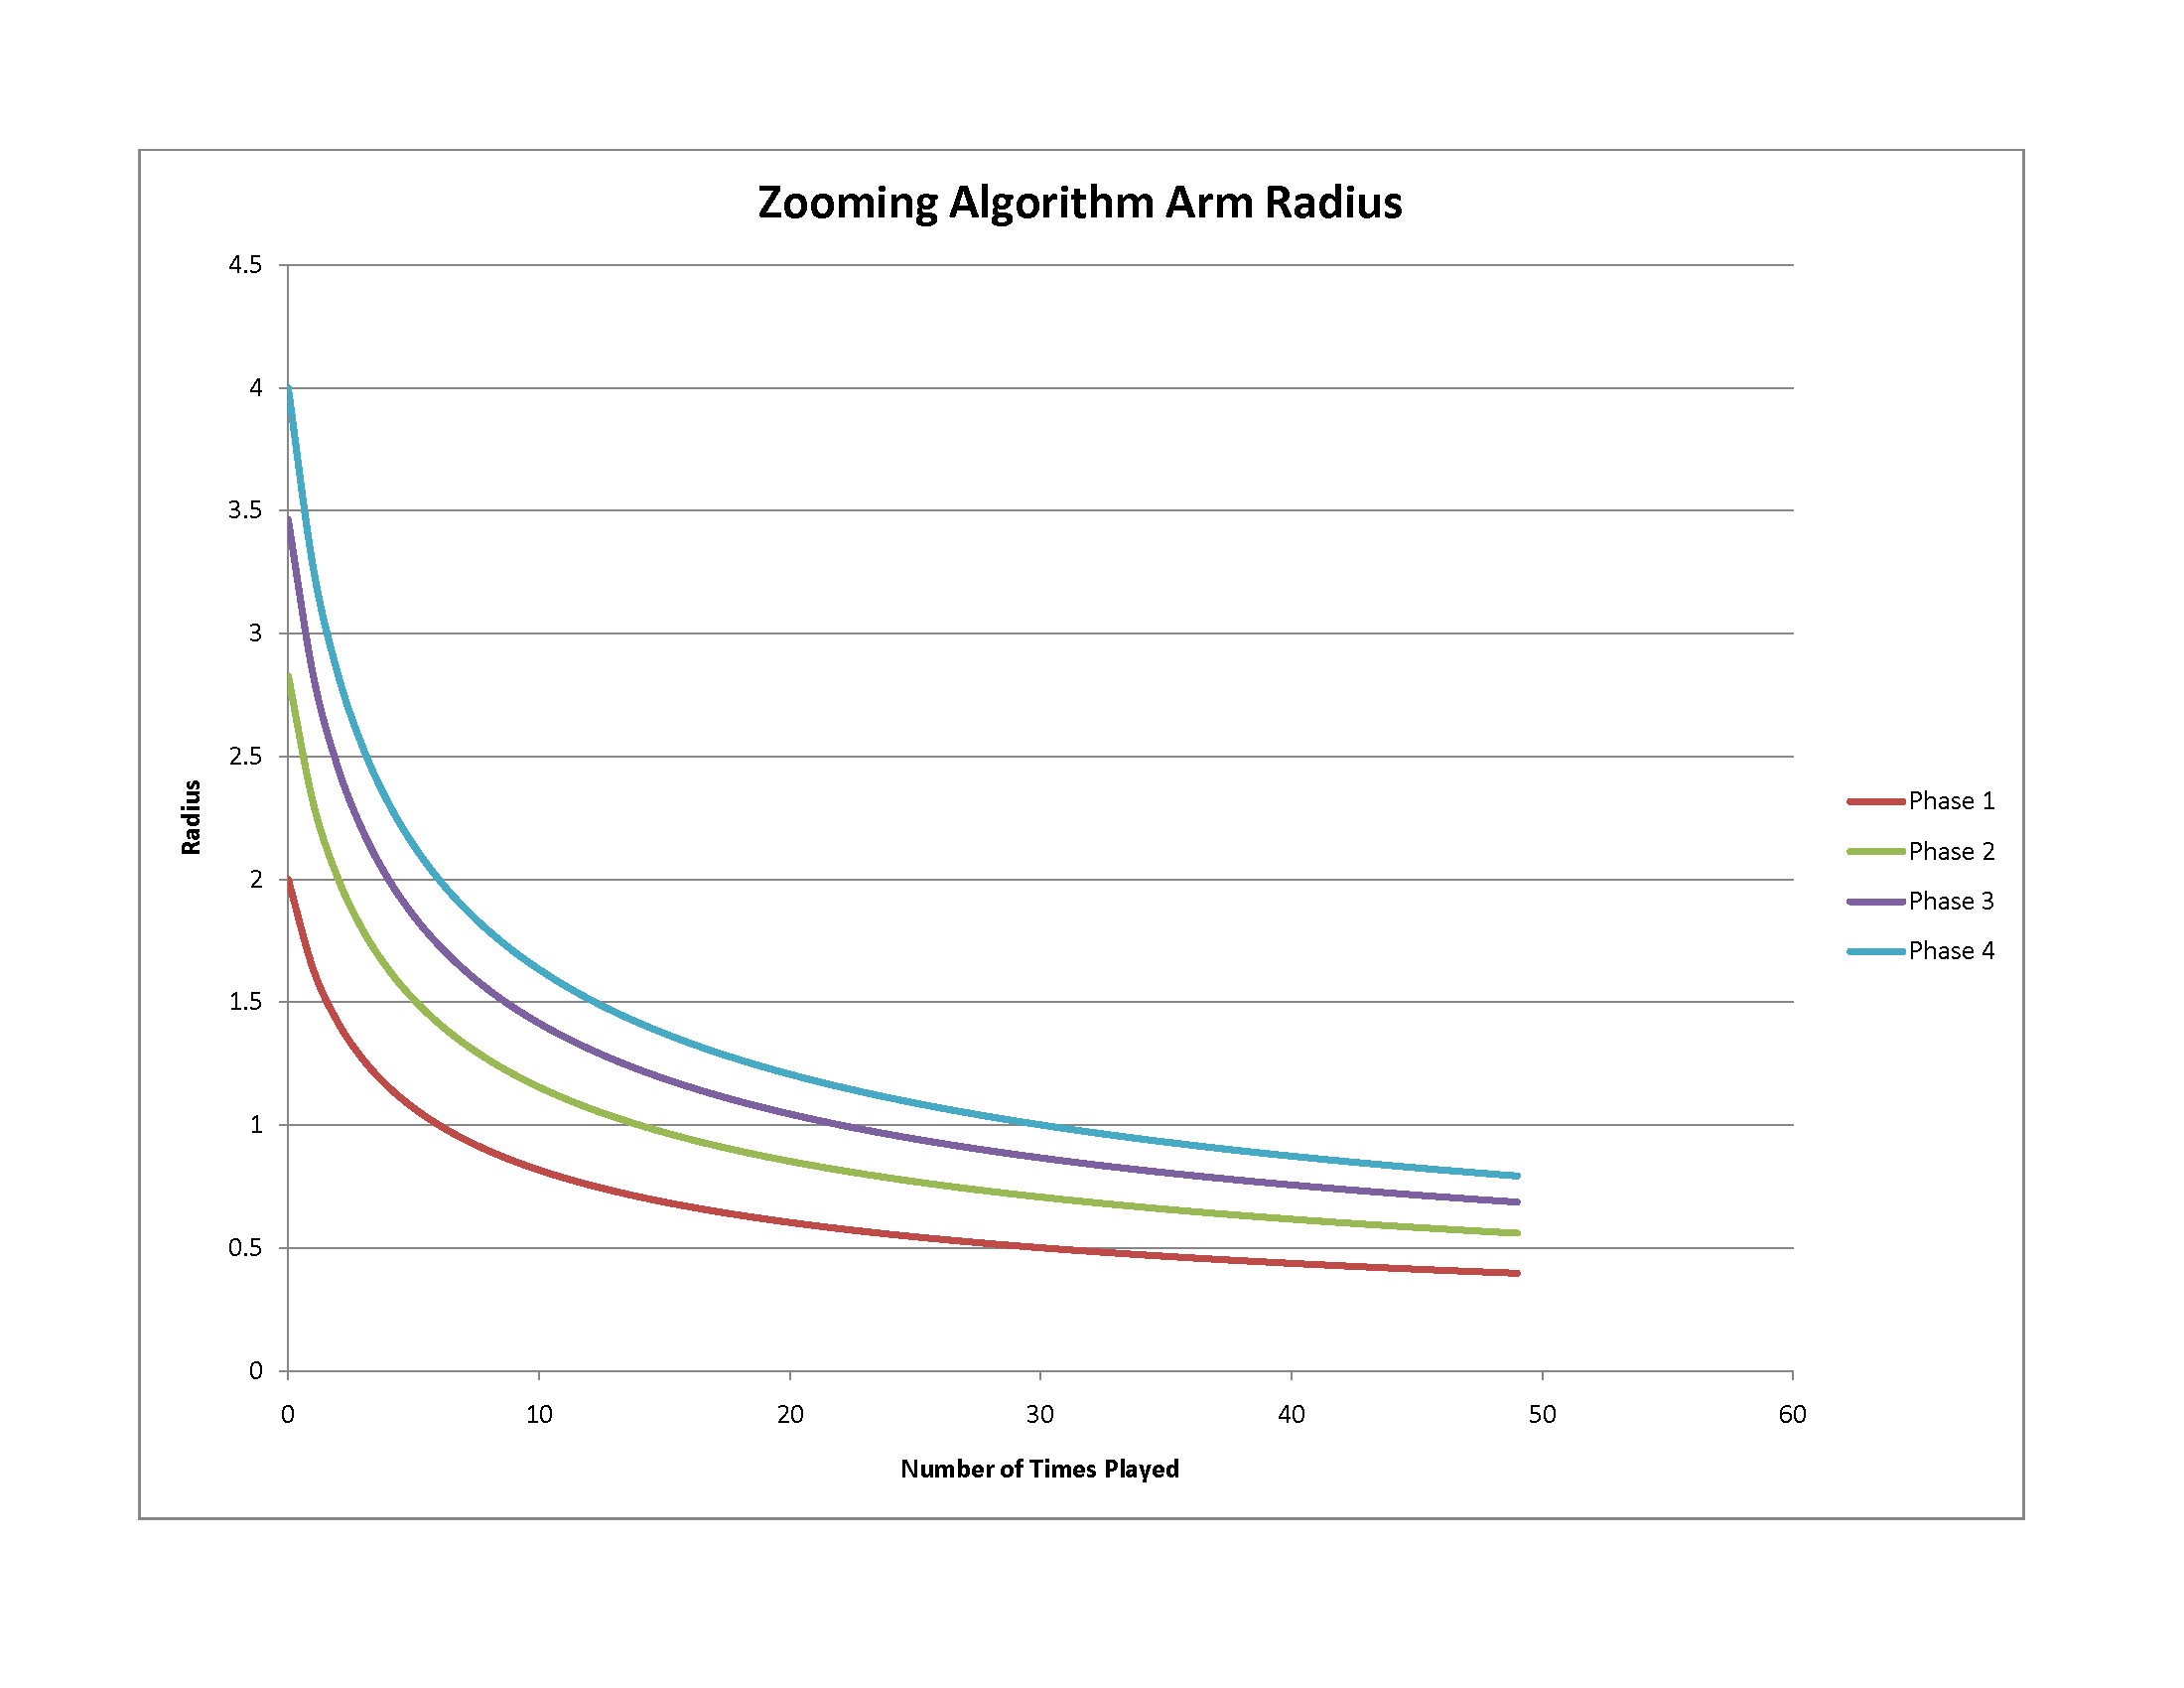
\includegraphics[width=5 in]{figures/ZoomingRadius.png}
     \caption{Arms cover less area the more they are played. The phase number only changes the scaling.}
     \label{fig:zoomphase}
  \end{center}
\end{figure}

Inbetween different phases, the Zooming Algorithm does not carry
over information. All that changes is $i_{ph}$. As $i_{ph}$ increases,
the index is effected increasingly more by how many times an arm has
been played. This means that earlier rounds have indices that are more
influenced by the $\mu_t(v)$, and will thus tend to exploit their earlier
finds more, while later rounds will perform more exploration before zeroing
in on the optimal arm. Given specific knowlege about the problem at hand,
this value could be optimized, allowing you to run the zooming algorithm
for a specific phase number. 

\begin{figure}[!ht]
  \begin{center}
    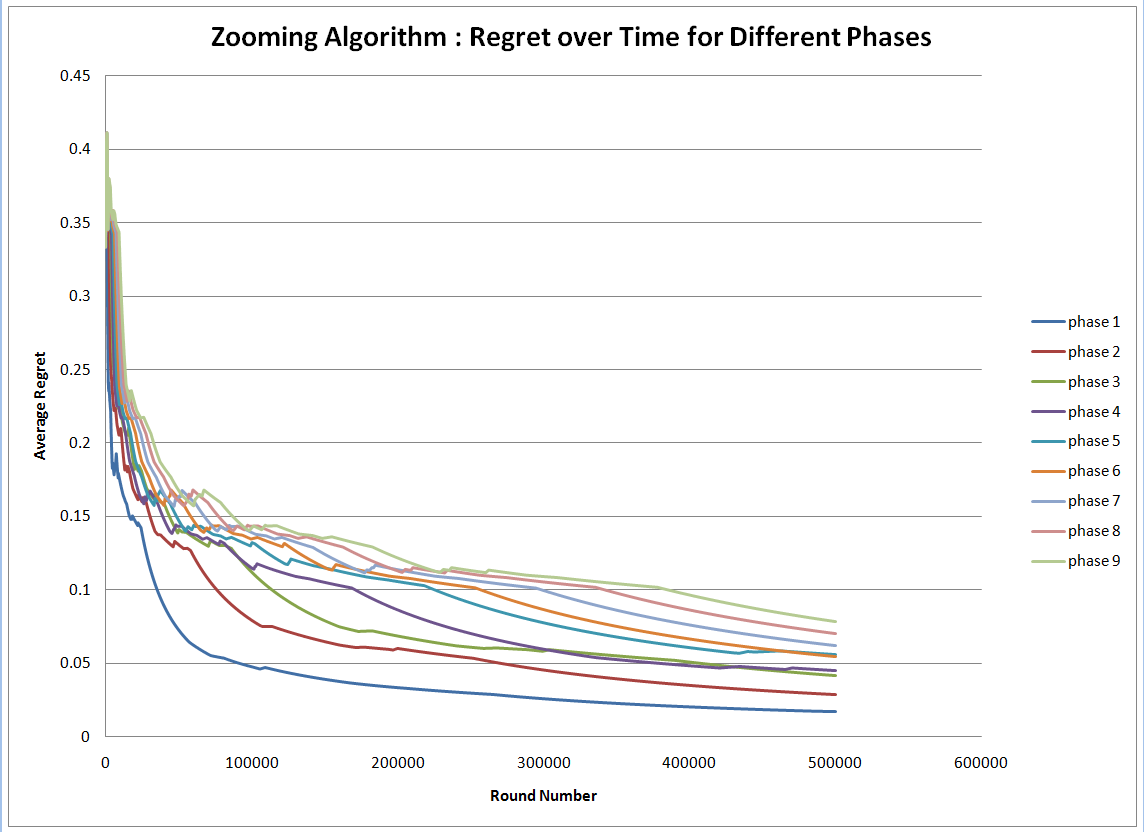
\includegraphics[width=5 in]{figures/Phase_Comparison.png}
     \caption{Here, the Zooming Algorithm was modified to run indefinitely on a specific phase number. As you can see, as a result of later phases doing more exploration, and having larger initial radii for their arms, later phases take longer to converge than earlier phases. The algorithm was run on a 2 dimensional domain from 0 to 1 where reward is maximized at the point $(.3,.3)$. Reward was given by $\frac{1}{1+\mathrm{d}(v,(.3,.3))}$}
     \label{fig:zoomphase}
  \end{center}
\end{figure}



The runtime of the Zooming Algorithm depends very heavily on how the
covering oracle chosen behaves. This can be problematic, since the problem
is np-complete for the problem of hypercube coverings  \cite{Hoffmann05acovering} . In high dimensions,
the oracle can become quite expensive.

%%%%%%%%%%%%%%%%%%%%%%%%%%%%%%%%%%%%%%%%%%%%%%%%%%%%%%%%%%%%%%%%%%%%%%%%%%%%%
\subsection{Discretization Algorithms}
To test the $\mathcal{X}$-armed and Zooming algorithms, we have implemented
the $\epsilon$-greedy, UCB1, and Exp3 finite-armed algorithms for
the case where whatever domain our bandit problem is over is discretized
into some finite number $K$ points.  In common to each algorithm is the
fact that the points are chosen randomly and uniformly from the domain.  The
intuition behind this choice is that, otherwise, it would be relatively easy
to construct a reward function that any discretization would do terribly
for, simply by ensuring that the peaks of the reward function did not occur
where the algorithm picked a point.  For example, if arms were chosen in
regular intervals from the interval [0,1], i.e. at the points 
$\frac{i}{K+1}$, with $1 \leq i \leq K$, then a reward function with a
sharp peak at 0 would be guaranteed to make any discretization algorithm
perform poorly.  Choosing the arms at random at least guarantees that there
is a chance of doing well.  A brief description of the particulars of 
each algorithm is now given.

\subsubsection{$\epsilon$-Greedy}
In round $t$, if $1 \leq t \leq K$ then play arm $t$.  Otherwise, play
randomly with probability $\epsilon$ and the arm with the best running
average otherwise.  We have implemented this algorithm using
$\epsilon = \frac{K}{t}$.

\subsubsection{UCB1}
In round $t$, if $1 \leq i \leq K$ then play arm $i$.  Otherwise, play
the arm that maximizes the quantity
\[
	\bar{r_i} + \sigma \sqrt{\frac{2 \log(t)}{p_i}}
\]
Where $\bar{r_i}$ is the average reward of arm $i$ so far, $p_i$ is the 
number of times arm $i$ has been played so far, and $\sigma$ is a parameter
that can be chosen to influence how much exploration is done.

\subsubsection{Exp3}
Initialize $w_i(1) = 1$ for all $1 \leq i \leq K$.  In round $t$, play
arm $i$ with probability
\[
	p_i(t) = \frac{\epsilon}{K} + (1 - \epsilon) \frac{w_i(t)}{\sum_j w_j(t)}
\]
With $i$ the arm that was played, update
\[
	w_i(t+1) = w_i(t)\gamma^{\frac{\epsilon r_i(t)}{K p_i(t)}}
\]
where $r_i(t)$ is the reward recieved, and set $w_j(t+1) = w_j(t)$ for all
other arms $j$.  $\gamma$ is a parameter that can be chosen to influence how
much exploration is done.  As in the $\epsilon$-greedy algorithm, we use
$\epsilon = \frac{K}{t}$.